\documentclass[twocolumn]{autart}

%% DOI and ARXIV Commands for Bib Files
% Written by Daniel Herber
% -----------------------------------------------
% one option is to use the 'note' field with this command
% -----------------------------------------------
% for example, if your doi is 10.2514/1.J052182
% then for the citation for the reference in your bib file, use
% note = "\doi{10.2514/1.J052182}",
% -----------------------------------------------
% for example, if your arxiv number is 0706.1234
% then for the citation for the reference in your bib file, use
% note = "\arxiv{0706.1234}",

% requires hyperref package for \href command
\usepackage{hyperref}

% doi command (use in bib file)
\newcommand{\doi}[1]{{doi:~\href{http://doi.org/#1}{#1}}\rmFullStop}

% arXiv command (use in bib file)
\newcommand{\arxiv}[1]{{arXiv:\href{https://arxiv.org/abs/#1}{#1}}\rmFullStop}

% command to remove full stop if the next character
\newcommand*{\rmFullStop}{\rmifnextchar{.}{}{}}

% command to check the next character and replace if present
% \rmifnextchar{X}{[removed text]}{[no X text]}
% if X is the next character, then it is removed and [removed text] is inserted
% otherwise, the character is not removed and [no X text] is inserted
% based on http://tex.stackexchange.com/questions/72827
\makeatletter
\newcommand{\rmifnextchar}[3]{%
  \begingroup
  \ltx@LocToksA{\endgroup#2}%
  \ltx@LocToksB{\endgroup#3}%
  \ltx@ifnextchar{#1}{%
    \def\next{\the\ltx@LocToksA}%
    \afterassignment\next
    \let\scratch= %
  }{%
    \the\ltx@LocToksB
  }%
}
\makeatother
%\RequirePackage{doi}
\usepackage[
	pdftitle={topi.link: The Northern/Southern Ontology},
	pdfsubject={topi.link: The Northern/Southern Ontology},
	pdfauthor={Florian Thiery},
	pdfkeywords={Linked Data, Semantic Reasoning, Vagueness, Conceptual Modeling}
]{hyperref}

\usepackage{graphicx}          % Include this line if your 
                               % document contains figures,
%\usepackage[dvips]{epsfig}    % or this line, depending on which
                               % you prefer.
\usepackage{verbatimbox}

\begin{document}

\begin{frontmatter}
%\runtitle{Insert a suggested running title}  % Running title for regular 
                                              % papers but only if the title  
                                              % is over 5 words. Running title 
                                              % is not shown in output.

\title{The SPARQL Unicorn: An introduction}
                                               

\author[FT]{Florian Thiery},
\author[SCS]{Sophie C. Schmidt},
\author[TH]{Timo Homburg},
\author[MT]{Martina Trognitz}

\address[FT]{ORCID: 0000-0002-3246-3531, Research Squirrel Engineers}
\address[SCS]{ORCID: 0000-0003-4696-2101, Research Squirrel Engineers}
\address[TH]{ORCID: 0000-0002-9499-5840, Research Squirrel Engineers}
\address[MT]{ORCID: 0000-0003-0485-6861, Research Squirrel Engineers}

          
\begin{keyword}                             
Linked Data; SPARQL; RDF; SPARQL Unicorn.
\end{keyword}

\begin{abstract}                         

What ist the SPARQL Unicorn? How can a unicorn help researchers handling and working with Linked Open Data resources? This working paper will give an overview on the SPARQL unicorn history, the main idea, developed tools and projects.

\end{abstract}

\end{frontmatter}

\section{The SPARQL Unicorn History}

The SPARQL Unicorn was born at the `Computer Applications and Quantitative Methods in Archaeology` conference 2019 in Kraków, Poland. As one of the important parts of scientific conferences, networking and knowledge exchange (here in the famous Stary Port), brought interesting to daylight: We all want to publish Open Daten and support volunteered community driven data collecting initiatives like Wikidata. 

\begin{figure}[!htb]
\begin{center}
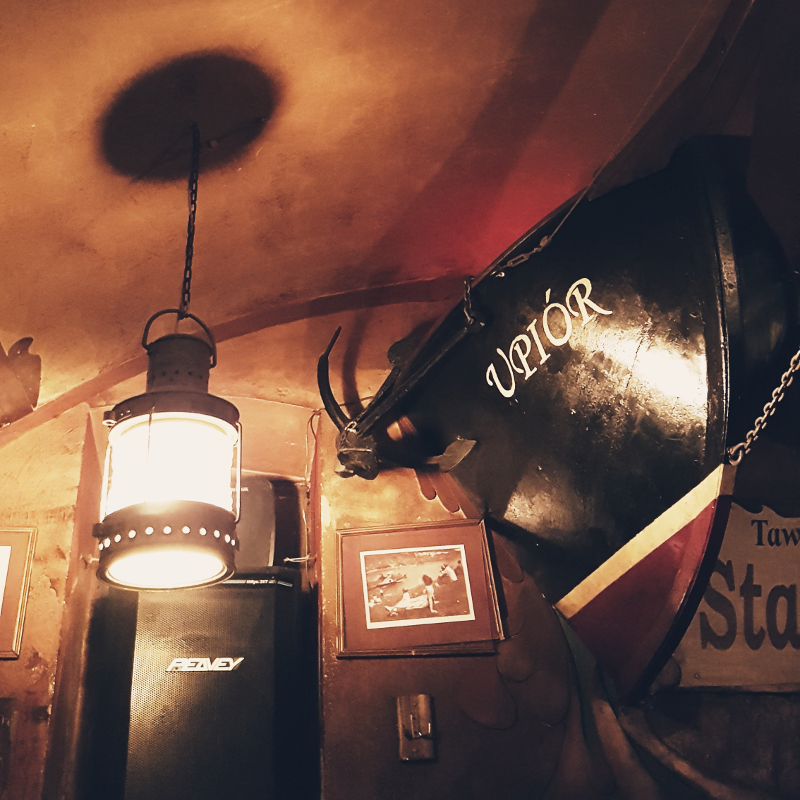
\includegraphics[width=6cm]{20190423_213750.jpg}
\caption{Stary Port, Kraków}
\label{rq1}
\end{center}
\end{figure}

But on the other hand there is a lack of user-friendly, easy to use and openly available tools, especially for Linked Open Data technologies and repositories as well as Wikidata itself. To overcome this bottleneck the SPARQL Unicorn may help. The Research Squirrel Engineers network and research group (RSE) was founded by Sophie Charlotte Schmidt, Martina Trognitz, Timo Homburg and Florian Thiery to bring this Unicorn to life. The Research Squirrels will develop and maintain all activities (e.g. tools, projects) according to the SPARQL Unicorn principles, other related applications as well as generating outreach and support activities to include the SPARQL unicorn into research and teaching. 

\section{The SPARQL Unicorn Idea}

\begin{figure}[!htb]
\begin{center}
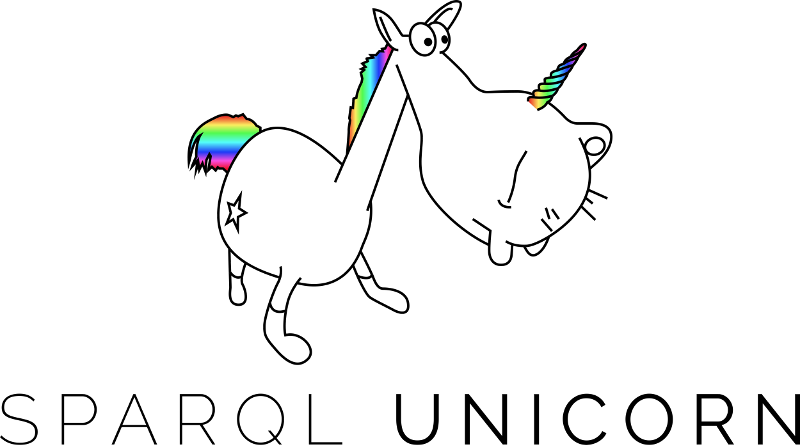
\includegraphics[width=6cm]{sparqlunicorn_logo.png}
\caption{SPARQL Unicorn}
\label{rq1}
\end{center}
\end{figure}

In humanities, databases as well as data modelling and their analyses play a central role. Some of these data(bases) are online available, open, accessible and hopefully linked to other datasets in the Linked Open Data Cloud. Nevertheless, there is one volunteered community driven Open Source Linked Data repository that recently gained momentum: Wikidata. We would like to propose the `SPARQL Unicorn` as a user friendly easy to use tool series for researchers working with Wikidata. The unicorn’s aim is to help researchers in using the community driven data from Wikidata and make it accessible to them without expertise in Semantics, Linked Open Data or SPARQL.

So, we propose the `SPARQL Unicorn principles`:

(1) Describe your data in well documented semantic structured open formats, acc. to the 5 Star data principles.

(2) Model, generate and publish your data as 5 Star Linked Open Data

(3) Publish your data in Wikidata and interlink them to other resources in the Linked Open Data Cloud

(4) Use existing tools to query Wikidata dynamically and to do real time data analysis and support developers or develop new tools to give people without any deeper knowledge in Linked Open Data (SPARQL Unicorn tools) the possibility to also do dynamical real time analysis

(5) Use Wikidata and the SPARQL Unicorn tools in your own research and promote the SPARQL Unicorn principles that other interested researchers in the community may start with principle 1!

\section{The SPARQL Unicorn Tools}

The set of SPARQL Unicorn tools is an open list for user-friendly Wikidata related tools developed and maintained by the Research Squirrel Engineers. If you are interested in a special topic do not hesitate to contact the squirrels. Today, a geospatial related QGIS plugin, the SPARQling Unicorn QGIS Plugin has been implemented and published. More tools, like a SPARQLing Unicorn R Package for statistical analysis is still under development.

\subsection{SPARQling Unicorn QGIS Plugin}

Tools for integrating geodata in the Semantic Web into classical desktop applications are missing. The SPARQLing Unicorn QGIS Plugin enables (GeoSPARQL) queries into selected triplestores and georelated SPARQL endpoints and processes the results for usage into QGIS for the geo community. Right now the plugin offers three functions:

\begin{figure}[!htb]
\begin{center}
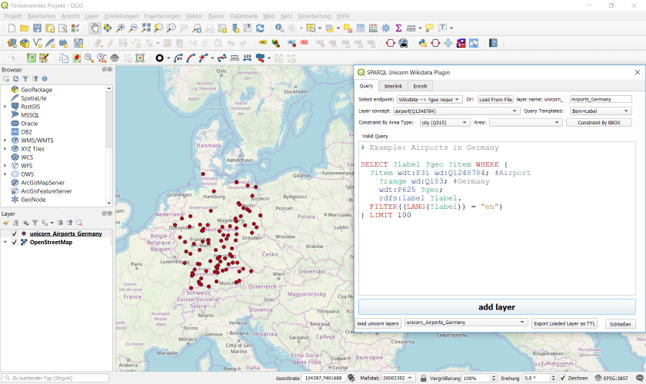
\includegraphics[width=8cm]{qgis1.png}
\caption{QGIS Plugin SPARQL Query}
\label{rq1}
\end{center}
\end{figure}

(1) Simplified querying of Semantic Web data sources. First, semantic databases, so-called SPARQL endpoints, are examined for geo-concepts. You can then request these with pre-generated SPARQL query patterns and if necessary, limit them with a bounding box. These functionalities do not require any knowledge of the SPARQL query language. Experts who are familiar with SPARQL can adapt the proposed queries according to their own wishes. The results of the queries are converted into GeoJSON layers so that they can be used directly in QGIS. The plugin thus offers the possibility of automatically generating simple queries such as `Give me all universities in BOUNDINGBOX` or `Give me all airports in COUNTRY X` and thus makes it easier to load dynamic contents of the linked data data repositories. 

\begin{figure}[!htb]
\begin{center}
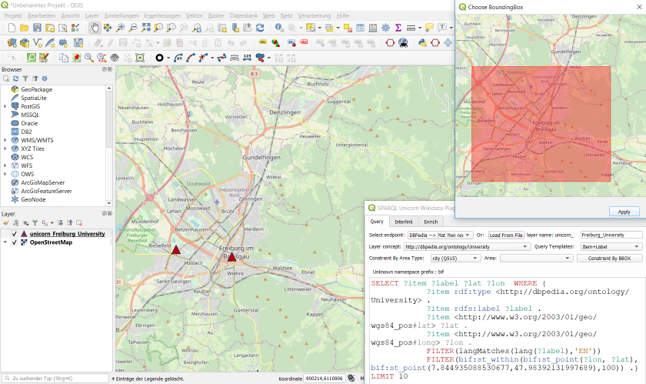
\includegraphics[width=8cm]{qgis2.png}
\caption{QGIS Plugin Bounding Box}
\label{rq1}
\end{center}
\end{figure}

(2) Enrichment of geodata. In addition to loading geodata from the Semantic Web, another interesting application is the enrichment of geodata with Semantic Web data. For this, correspondences between the respective columns of the table of the geodata set must be found and specified in the Semantic Web. Alternatively, the table can be expanded with a new column that is completely extracted from the Semantic Web. Subsequently, enrichment can be carried out according to various strategies such as overwriting and adding geodata, merging the results or decision of the user. The latter may be necessary especially in the event of conflicts in the data from the two data sources. The geodata set can now be exported in any geospatial format available in QGIS. An example of such an enrichment is the use of founding years and the attribute 'disability friendliness' of schools from Wikidata for a data set of schools which was extracted from OpenStreetMap. While the key "wheelchair" already exists in OpenStreetMap and can possibly be completed by Semantic Web data, the attribute `inception` is less common in OpenStreetMap and can possibly be generated again. The map can then e.g. be colored according to the date of foundation.

(3) Enrichment and conversion of RDF data. The third function of the plugin is the enrichment of RDF data for the linked data community. For this, geodata sets can be loaded into the plugin and semantic web correspondences can be specified for the data set. The result of this mapping process is a linked data set in e.g. RDF, which is inserted into a semantic database, a triple store and can thus be made available in the LOD cloud. Since our plugin also supports the import of RDF files in various formats in addition to querying SPARQL endpoints, this functionality can also be used to re-project RDF data via the detour as a QGIS layer. So, we are also contributing to the better handling of geodata for the Semantic Web Community.

\section{The SPARQL Unicorn Projects}

The Research Squirrel Engineers would like to bring the SPARQL Unicorn principles and the SPARQL Unicorn tools to life and therefore created some ancient studies related research projects where this digital method approach related to Wikidata and Linked Open Data is followed consistently. One project is the \textbf{Ogi Ogham Project}, that concentrates on more or less Irish (British) Ogham Stones containing Ogham Inscriptions. Another project that will come up is the \textbf{Lasse-Olav Rockart Project} which deals with prehistoric rock art in the Scandinavian countries, especially in the north of Norway, in Alta.

\subsection{Ogi Ogham Project}

Stones carrying Ogham inscriptions are found in Ireland and the western part of Britain (Wales and Scotland). Ogham stones mainly served as memorials and/or boundary markers as well as indicators of land ownership and contained relationships as well as personal attributes. They date from the 4th century AD to the 9th century AD MacManus (1997)\cite{macmanus_guide_1997}. Probably the most complete standard reference is found in Macalister (1945, 1949)\cite{macalister_corpus_1945}\cite{macalister_corpus_1949}, who established the CIIC scheme. Ogham inscriptions contain formula words like MAQI (son) or MUCOI (tribe/sept). The Irish personal name nomenclature reveals details of early Gaelic society, e.g. CUNA (wolf/hound) or CATTU (battle), details in Thiery (2020)\cite{thiery_ogham_2020} and MacManus (1997)\cite{macmanus_guide_1997}.

\begin{figure}[!htb]
\begin{center}
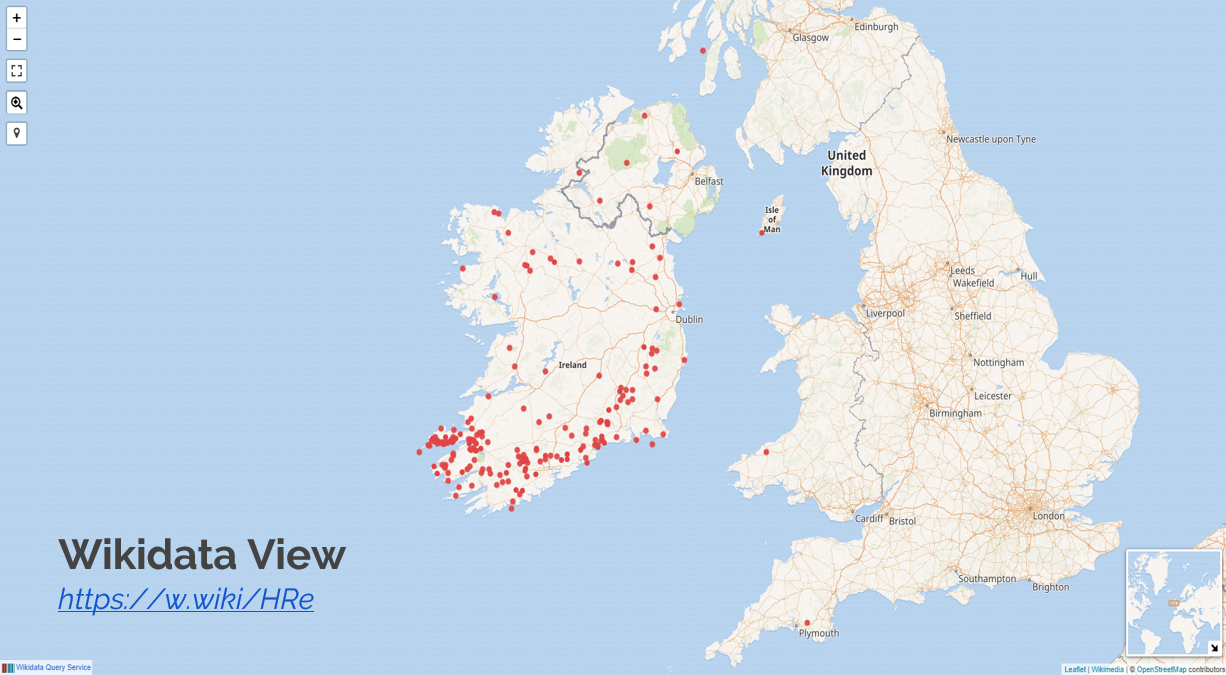
\includegraphics[width=8cm]{ogham.png}
\caption{Ogham Stones in Wikidata}
\label{rq1}
\end{center}
\end{figure}

The idea of the Ogi Ogham Project is to provide the Ogham stones, their content, the relationships of the people noted on stones, their tribal affiliations and other metadata as Linked Open Data; thus enabling semantic research processing by the scientific community. The Research Squirrel Engineers do this job, so Linked Ogham Stones allow the following research questions to be addressed by linking knowledge and enriching it: (i) classification of stones (e.g. family hierarchy) and (ii) visualisation of relationships in maps generated by LOD. As a fundament for the analyses, the projects relies on a Wikidata retro-digitisation of the CIIC Corpus by Macalister (1945, 1949), EPIDOC data of the Ogham in 3D project and on the Celtic Inscribed Stones Project (CISP\footnote{https://www.ucl.ac.uk/archaeology/cisp/database/} ) database.

\subsection{Lasse-Olav Rockart Project}

In 1973 more than 6000 prehistoric carvings (rock art, petroglyphs) have been found (4200 BC to around 500 BC) in several sites\footnote{http://altarockart.no/}  around the municipality of Alta in the county of Finnmark in northern Norway. The sites Jiepmaluokta , Storsteinen, Kåfjord, Amtmannsnes and Transfarelv, were placed on the UNESCO list of World Heritage Sites on 3rd December 1985 and it is Norway's only prehistoric World Heritage Site. Here, the carvings show a culture of hunter-gatherers that was able to control herds of reindeer, was adept at boat building and fishing and practiced shamanistic rituals involving bear worship and other venerated animals. The rock art of Alta is also well documented in a digital archive\footnote{http://altarockart.no/fotoweb/archives/5002-Browse-in-English/} containing thousands of digital pictures and semantic descriptions.

\begin{figure}[!htb]
\begin{center}
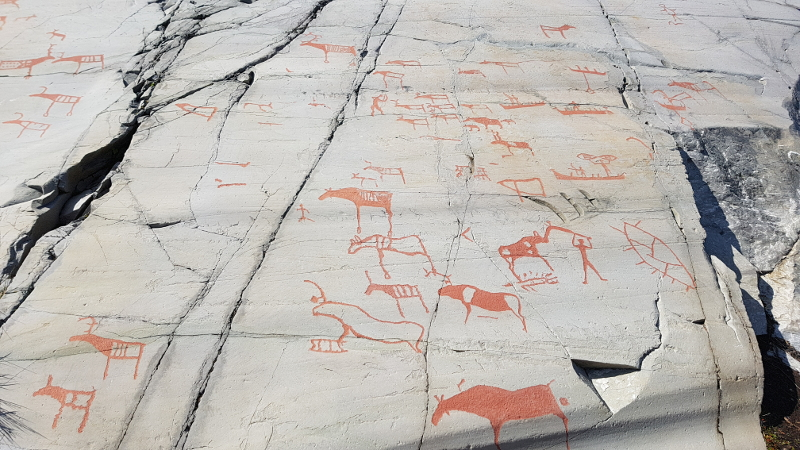
\includegraphics[width=8cm]{20190616_134048.jpg}
\caption{Rockart in Alta, Norway}
\label{rq1}
\end{center}
\end{figure}

The idea of the Lasse-Olav Rockart Project is to provide the carvings and their content as Linked Open Data. The Research Squirrel Engineers will model the data according to the SPARQL Unicorn principles and provide the research data in Wikidata.

\section{SPARQL Unicorn’s Outlook}

As you can see, the SPARQL Unicorn was born in 2019 and is doing its first careful steps into the Linked Open Data and Digital Humanities Community. Help us and promote the SPARQL Unicorn principles, use Wikidata, use and develop SPARQL Unicorn tools! The Research Squirrel Engineers look forward to every new Research Squirrel interested in unicorns!

\bibliographystyle{IEEEtran}
\bibliography{autosam}

\end{document}